
\section{ Introduction to Octave}
\begin{figure}[ht]
	\centering 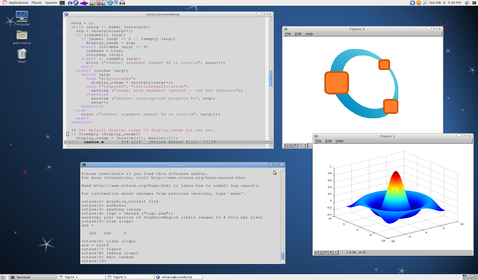
\includegraphics[scale=.50]{input/images/O1.png}
	\caption{Documentation using Doxygen (main page)}
\end{figure}

 GNU Octave is a high-level interpreted language, primarily intended for numerical computations. It provides capabilities for the numerical solution of linear and nonlinear problems, Image Processing and for performing other numerical experiments. It also provides extensive graphics capabilities for data visualization and manipulation. Octave is normally used through its interactive command line interface, but it can also be used to write non-interactive programs. The Octave language is quite similar to Matlab so that most programs are easily portable.

 Octave is distributed under the terms of the GNU General Public License.\\ 
 
 \textbf{GNU/Linux systems}
 
 Executable versions of Octave for GNU/Linux systems are provided by the individual distributions. Distributions known to package Octave include: Debian, Fedora, Gentoo, and SuSE. These packages are created by volunteers. The delay between an Octave source release and the availability of a package for a particular GNU/Linux distribution varies. The Octave project has no control over that process. 
 BSD systems\\
 
 Executable versions of Octave for BSD systems are provided by the individual distributions. Both FreeBSD and OpenBSD have Octave packages. These packages are created by volunteers. The delay between an Octave source release and the availability of a package for a particular GNU/Linux distribution varies. The Octave project has no control over that process.\\
 
 \textbf{OS X}

 The Wiki has some instructions for installing Octave on OS X systems.\\
 
\textbf{Windows}
 
 Windows binaries with corresponding source code can also be downloaded.
 
 \textbf{Sources}
 
 The latest released version of Octave is 4.3 released in July,2016.
 
  The simplest way to compile this package is:
 \begin{itemize}
 
\item 'cd' to the directory containing the package's source code and type './configure' to configure the package for your system.
 
Running 'configure' might take a while.  While running, it prints
 some messages telling which features it is checking for.
 
\item Type 'make' to compile the package.
 
\item Optionally, type 'make check' to run any self-tests that come with
 the package, generally using the just-built uninstalled binaries.
 
\item Type 'make install' to install the programs and any data files and
 documentation.  When installing into a prefix owned by root, it is
 recommended that the package be configured and built as a regular
 user, and only the 'make install' phase executed with root
 privileges.
 
\item Optionally, type 'make installcheck' to repeat any self-tests, but
 this time using the binaries in their final installed location.
 This target does not install anything.  Running this target as a
 regular user, particularly if the prior 'make install' required
 root privileges, verifies that the installation completed
 correctly.
 
\item You can remove the program binaries and object files from the
 source code directory by typing 'make clean'.  To also remove the
 files that 'configure' created (so you can compile the package for
 a different kind of computer), type 'make distclean'.  There is
 also a 'make maintainer-clean' target, but that is intended mainly
 for the package's developers.  If you use it, you may have to get
 all sorts of other programs in order to regenerate files that came
 with the distribution.
 
 \item Often, you can also type 'make uninstall' to remove the installed
 files again.  In practice, not all packages have tested that
 uninstallation works correctly, even though it is required by the
 GNU Coding Standards.
 
\item Some packages, particularly those that use Automake, provide 'make
 distcheck', which can by used by developers to test that all other
 targets like 'make install' and 'make uninstall' work correctly.
 This target is generally not run by end users.
\end{itemize}


